\documentclass[14pt,a4paper]{extarticle}
\usepackage[T1]{fontenc}
\usepackage[utf8]{inputenc}
\usepackage[scaled]{helvet}
\renewcommand{\familydefault}{\sfdefault}
\usepackage{amsmath}
\usepackage{sansmath}
\sansmath
\usepackage[a4paper,hmargin=2cm,vmargin=1.6cm]{geometry}
\usepackage{tikz}
\usetikzlibrary{angles,quotes,patterns}
\usepackage{array}
\pagestyle{empty}
% Zweite Seite: 5-mm-Kästchen, 1 cm Rand
\newcommand{\kaestchen}{\newpage\null\begin{tikzpicture}[remember picture,overlay]
\begin{scope}[shift={(current page.south west)}]\draw[step=5mm, black!45, line width=0.3pt] (1cm,1cm) grid (20cm,28.5cm);\draw[black!45, line width=0.3pt] (1cm,1cm) rectangle (20cm,28.5cm);\end{scope}
\end{tikzpicture}}
\setlength{\parindent}{0pt}
\hyphenpenalty=10000

% Nur Schwarz und Grau, die Blätter werden schwarz-weiß kopiert.
% Winkelfläche: Scheitel, Startwinkel, Endwinkel, Füllung, Name
\newcommand{\wk}[5]{\fill[#4] (#1) -- ++(#2:0.62) arc (#2:#3:0.62) -- cycle; \node at ([shift={({(#2+#3)/2}:1.02)}]#1) {\large$#5$};}
% Die vier Winkel einer Kreuzung: Scheitel, Richtung der schrägen Geraden, Index
\newcommand{\vier}[3]{%
\wk{#1}{0}{#2}{gray!45}{\alpha_{#3}}\wk{#1}{#2}{180}{gray!15}{\beta_{#3}}%
\wk{#1}{180}{#2+180}{gray!45}{\gamma_{#3}}\wk{#1}{#2+180}{360}{gray!15}{\delta_{#3}}}
% Lücke zum Eintragen
\newcommand{\lu}{\rule{1.1cm}{0.4pt}}
\newcommand{\nr}[1]{{\Large\bfseries #1}\quad}
\renewcommand{\arraystretch}{1.35}
\raggedright

\begin{document}

{\LARGE\bfseries Üben: Winkel an Geraden und Parallelen\par}
\vspace{0.25cm}

\begin{tabular}{|l|*{6}{>{\centering\arraybackslash}p{1.45cm}|}>{\centering\arraybackslash}p{2.6cm}|}
\hline
 & 1 & 2 & 3 & 4 & 5 & 6 & richtig\\\hline
Start & & & & & & & \\\hline
Schluss & & & & & & & \\\hline
\end{tabular}

\vspace{0.55cm}

\begin{minipage}[t]{0.37\textwidth}
\nr{1} Trage die Winkel ein.\par\bigskip\medskip
\centering
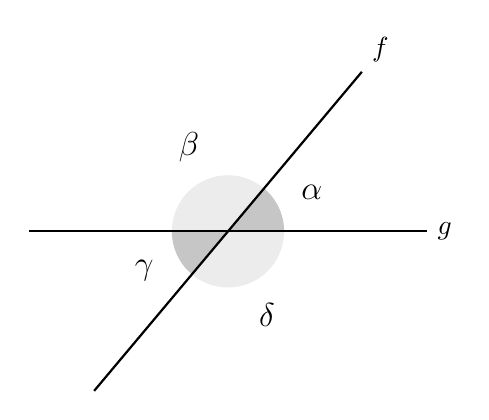
\begin{tikzpicture}[scale=1.15, baseline=(current bounding box.north)]
  \coordinate (S) at (0,0);
  \wk{S}{0}{50}{gray!45}{\alpha}\wk{S}{50}{180}{gray!15}{\beta}\wk{S}{180}{230}{gray!45}{\gamma}\wk{S}{230}{360}{gray!15}{\delta}
  \draw[thick] (-2.2,0) -- (2.2,0) node[right] {$g$};
  \draw[thick] (230:2.3) -- (50:2.3) node[above right] {$f$};
\end{tikzpicture}\par\medskip
\raggedright
\begin{tabular}{@{}l@{\qquad}l@{}}
$\alpha = 50^\circ$ & $\beta = $ \lu\\
$\gamma = $ \lu & $\delta = $ \lu
\end{tabular}
\end{minipage}\hfill
\begin{minipage}[t]{0.6\textwidth}
\raggedright\nr{2} $g \parallel h$. Trage die Winkel ein. Schreibe zu drei Winkeln die Regel auf die Rückseite.\par\medskip
\centering
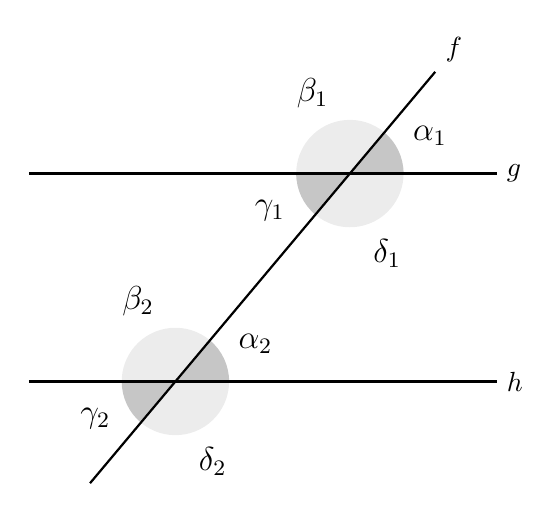
\begin{tikzpicture}[scale=1.1, baseline=(current bounding box.north)]
  \coordinate (G) at (1.007,1.2); \coordinate (H) at (-1.007,-1.2);
  \vier{G}{50}{1}\vier{H}{50}{2}
  \draw[thick] (-2.7,1.2) -- (2.7,1.2) node[right] {$g$};
  \draw[thick] (-2.7,-1.2) -- (2.7,-1.2) node[right] {$h$};
  \draw[thick] (230:3.1) -- (50:3.1) node[above right] {$f$};
\end{tikzpicture}\par\medskip
\raggedright
\begin{tabular}{@{}l@{\hspace{0.45em}}l@{\hspace{0.45em}}l@{}}
$\alpha_1 = $ \lu & $\beta_1 = 130^\circ$ & $\gamma_1 = $ \lu\\
$\delta_1 = $ \lu & $\alpha_2 = $ \lu & $\beta_2 = $ \lu\\
$\gamma_2 = $ \lu & $\delta_2 = $ \lu &
\end{tabular}
\end{minipage}

\vspace{0.3cm}

\nr{3} Zeichne auf der Rückseite zwei Parallelen $g$ und $h$ und eine schräge Gerade $f$. Miss einen Winkel und berechne die anderen sieben.\par

\vspace{0.3cm}

\begin{minipage}[c]{0.62\textwidth}
\nr{4} $g \parallel h$. Trage die Winkel ein.\par\medskip
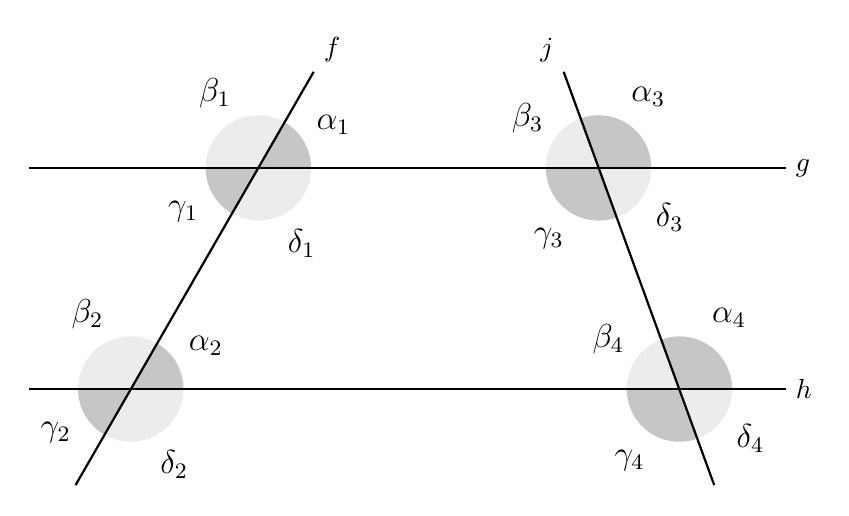
\begin{tikzpicture}[scale=1.08]
  \coordinate (A) at (-1.9,1.3); \coordinate (B) at (-3.4,-1.3);
  \coordinate (C) at (2.1,1.3); \coordinate (D) at (3.05,-1.3);
  \vier{A}{60}{1}\vier{B}{60}{2}\vier{C}{110}{3}\vier{D}{110}{4}
  \draw[thick] (-4.6,1.3) -- (4.3,1.3) node[right] {$g$};
  \draw[thick] (-4.6,-1.3) -- (4.3,-1.3) node[right] {$h$};
  \draw[thick] (-4.05,-2.43) -- (-1.25,2.43) node[above right] {$f$};
  \draw[thick] (3.46,-2.43) -- (1.69,2.43) node[above left] {$j$};
\end{tikzpicture}
\end{minipage}\hfill
\begin{minipage}[c]{0.37\textwidth}
\renewcommand{\arraystretch}{1.3}\begin{tabular}{@{}l@{\hspace{0.6em}}l@{}}
$\alpha_1 = 60^\circ$ & $\alpha_3 = 110^\circ$\\
$\beta_1 = $ \lu & $\beta_3 = $ \lu\\
$\gamma_1 = $ \lu & $\gamma_3 = $ \lu\\
$\delta_1 = $ \lu & $\delta_3 = $ \lu\\
$\alpha_2 = $ \lu & $\alpha_4 = $ \lu\\
$\beta_2 = $ \lu & $\beta_4 = $ \lu\\
$\gamma_2 = $ \lu & $\gamma_4 = $ \lu\\
$\delta_2 = $ \lu & $\delta_4 = $ \lu
\end{tabular}
\end{minipage}

\vspace{0.3cm}

\nr{5} $f$ schneidet $g$ und $h$. Zwei Wechselwinkel sind beide $80^\circ$ groß. Sind $g$ und $h$ parallel? Begründe.\par

\vspace{0.3cm}

\nr{6} $g \parallel h$ und $f \parallel j$. Ein Winkel ist $70^\circ$ groß. Zeichne auf der Rückseite und bestimme alle sechzehn Winkel.

\kaestchen
\end{document}
